%%%%%%%%%%%%%%%%%%%%%%%%%%%%%%%%%%%%%%%%%
% HW Template
% LaTeX Template
% Version 1.0 (19/10/18)
% Modified by
% Erdem TUNA
% Halil TEMURTAŞ 
% Enes TAŞTAN 
%%%%%%%%%%%%%%%%%%%%%%%%%%%%%%%%%%%%%%%%%
%
%----------------------------------------------------------------------------------------
%	PACKAGES AND OTHER DOCUMENT CONFIGURATIONS
%----------------------------------------------------------------------------------------
\documentclass[a4paper,12pt]{article}
%-----packages------
\usepackage[a4paper, total={6.2in, 8.5in}]{geometry}
\usepackage[english]{babel}
\usepackage[utf8x]{inputenc}
\usepackage{amsmath}
\usepackage{mathtools}
\usepackage{graphicx}
\usepackage[colorinlistoftodos]{todonotes}
\usepackage{gensymb} % this could be problem
\usepackage{float}
\usepackage{fancyref}
\usepackage{subcaption}
\usepackage[toc,page]{appendix} %appendix package
\usepackage{xcolor}
\usepackage{listings}
\usepackage{xspace}
\usepackage{amssymb}
\usepackage{nicefrac}
\usepackage{gensymb}
\usepackage{fancyhdr}
\usepackage{blindtext}  % for dummy text, use \blindtext or \BlindText
\usepackage{lipsum}    % for dummy text, use \lipsum[3-56]
\usepackage[final]{pdfpages}  % pdf include
\usepackage{array} %allows more options in tables
\usepackage{pgfplots,pgf,tikz} %coding plots in latex
\usepackage{capt-of} % allows caption outside the figure environment
\usepackage[export]{adjustbox} %more options for adjusting the images
\usepackage{multicol,multirow,slashbox} % allows tables like table1
%\usepackage[hyperfootnotes=false]{hyperref} % clickable references
\usepackage{epstopdf} % useful when matlab is involved
%\usepackage{placeins} % prevents the text after figure to go above figure with \FloatBarrier 
%\usepackage{listingsutf8,mcode} %import .m or any other code file mcode is for matlab highlighting

%-----end of packages

%-----specifications-----
\definecolor{mGreen}{rgb}{0,0.6,0} % for python
\definecolor{mGray}{rgb}{0.5,0.5,0.5}
\definecolor{mPurple}{rgb}{0.58,0,0.82}
\definecolor{mygreen}{RGB}{28,172,0} % color values Red, Green, Blue for matlab
\definecolor{mylilas}{RGB}{170,55,241}

\setcounter{secnumdepth}{5} % how many sectioning levels to assign numbers to
\setcounter{tocdepth}{5}    % how many sectioning levels to show in ToC

\lstdefinestyle{CStyle}{
	commentstyle=\color{mGreen},
	keywordstyle=\color{magenta},
	numberstyle=\tiny\color{mGray},
	stringstyle=\color{mPurple},
	basicstyle=\footnotesize,
	breakatwhitespace=false,         
	breaklines=true,
	frame=single,
	rulecolor=\color{black!40},                 
	captionpos=b,                    
	keepspaces=true,                 
	numbers=left,                    
	numbersep=5pt,                  
	showspaces=false,                
	showstringspaces=false,
	showtabs=false,                  
	tabsize=2,
	language=C
}

\lstset{language=Matlab,%
	%basicstyle=\color{red},
	breaklines=true,%
	frame=single,
	rulecolor=\color{black!40},
	morekeywords={matlab2tikz},
	keywordstyle=\color{blue},%
	morekeywords=[2]{1}, keywordstyle=[2]{\color{black}},
	identifierstyle=\color{black},%
	stringstyle=\color{mylilas},
	commentstyle=\color{mygreen},%
	showstringspaces=false,%without this there will be a symbol in the places where there is a space
	numbers=left,%
	numberstyle={\tiny \color{black}},% size of the numbers
	numbersep=9pt, % this defines how far the numbers are from the text
	emph=[1]{for,end,break},emphstyle=[1]\color{red}, %some words to emphasise
	%emph=[2]{word1,word2}, emphstyle=[2]{style},    
}


\tikzset{
	desicion/.style={
		diamond,
		draw,
		text width=4em,
		text badly centered,
		inner sep=0pt
	},
	block/.style={
		rectangle,
		draw,
		text width=10em,
		text centered,
		rounded corners
	},
	cloud/.style={
		draw,
		ellipse,
		minimum height=2em
	},
	descr/.style={
		fill=white,
		inner sep=2.5pt
	},
	connector/.style={
		-latex,
		font=\scriptsize
	},
	rectangle connector/.style={
		connector,
		to path={(\tikztostart) -- ++(#1,0pt) \tikztonodes |- (\tikztotarget) },
		pos=0.5
	},
	rectangle connector/.default=-2cm,
	straight connector/.style={
		connector,
		to path=--(\tikztotarget) \tikztonodes
	}
}

\tikzset{
	desicion/.style={
		diamond,
		draw,
		text width=4em,
		text badly centered,
		inner sep=0pt
	},
	block/.style={
		rectangle,
		draw,
		text width=10em,
		text centered,
		rounded corners
	},
	cloud/.style={
		draw,
		ellipse,
		minimum height=2em
	},
	descr/.style={
		fill=white,
		inner sep=2.5pt
	},
	connector/.style={
		-latex,
		font=\scriptsize
	},
	rectangle connector/.style={
		connector,
		to path={(\tikztostart) -- ++(#1,0pt) \tikztonodes |- (\tikztotarget) },
		pos=0.5
	},
	rectangle connector/.default=-2cm,
	straight connector/.style={
		connector,
		to path=--(\tikztotarget) \tikztonodes
	}
}
%-----end of specifications-----


%----commands----
\newcommand\nd{\textsuperscript{nd}\xspace}
\newcommand\rd{\textsuperscript{rd}\xspace}
\newcommand\nth{\textsuperscript{th}\xspace} %\th is taken already
\newcommand{\specialcell}[2][c]{ \begin{tabular}[#1]{@{}c@{}}#2\end{tabular}} % for too long table lines

\newcommand{\blankpage}{
	\- \\[9cm]	
	{ \centering \textit{This page intentionally left blank.} \par }
	\- \\[9cm]
}% For Blank Page

\makeatletter
\renewcommand\paragraph{\@startsection{paragraph}{4}{\z@}%
	{-2.5ex\@plus -1ex \@minus -.25ex}%
	{1.25ex \@plus .25ex}%
	{\normalfont\normalsize\bfseries}}
\makeatother
%-----end of commands-----


\pagestyle{fancy}
\fancyhead[LO,LE]{Halil TEMURTAŞ / 2094522   }
\fancyhead[RO,RE]{November 23,2018}
\fancyfoot[RO,RE]{
\includegraphics[width=2.7cm]{images/eelogo}}

\begin{document}
\begin{center}
	\textbf{\large EE402 Discrete Time Systems \\[0.2cm] MP-4} \\
\end{center}


\begin{enumerate}
	\item 
		
		$$ G_{OL}=K_p\frac{0.1275(z+1)}{z^2-2.255z+1} $$
		
		$$ 	G_{OL}=K_p\frac{0.1275(z+1)}{(z-1.648)(z-0.606)} $$
		
		Let us find break in/away points		
		
		$$ \frac{d}{d\sigma}\frac{1}{G_{OL}(\sigma)}=\sigma^2 +2\sigma-3.25=0$$
		
		$$ \sigma_{1,2}=1,06\ \& \ 3,06$$
		
		\lstinputlisting[language=Matlab,firstline=1, lastline=5]{MP4_upd.m}
	
	\begin{figure}[H]
			\center
			\setlength{\unitlength}{\textwidth} 
		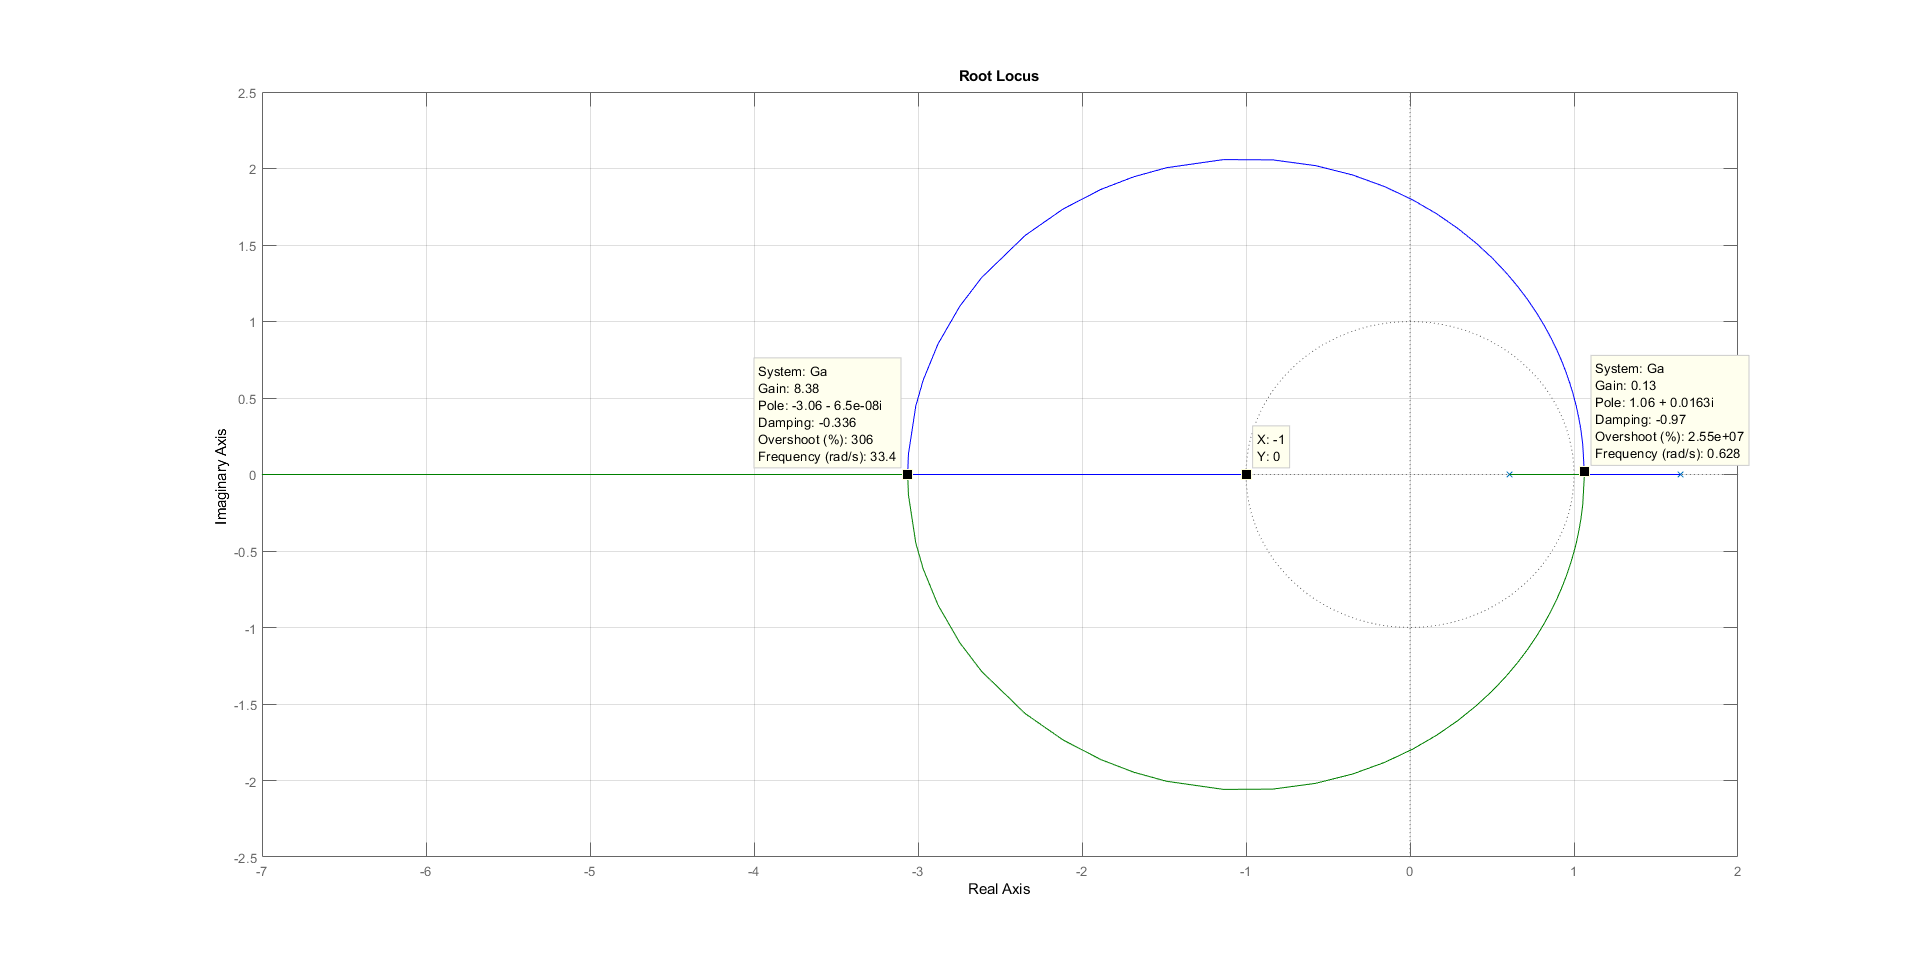
\includegraphics[width=1.0\unitlength]{images/1}
  		\caption{\label{fig:a}-}
	\end{figure}
	
	\item 
		
		$$ G_{OL}=K_p\frac{0.1275(z+1)}{z^2-1.215z-0.04} $$
		
		$$ 	G_{OL}=K_p\frac{0.1275(z+1)}{(z-1.247)(z+0.032)} $$
		

		Let us find break in/away points		
		
		$$ \frac{d}{d\sigma}\frac{1}{G_{OL}(\sigma)}=\sigma^2 +2\sigma-1.275=0$$		
		
		$$ \sigma_{1,2}=0,47\ \& \ -2,474$$
		
		\lstinputlisting[language=Matlab,firstline=9, lastline=13]{MP4_upd.m}
	
	\begin{figure}[H]
			\center
			\setlength{\unitlength}{\textwidth} 
		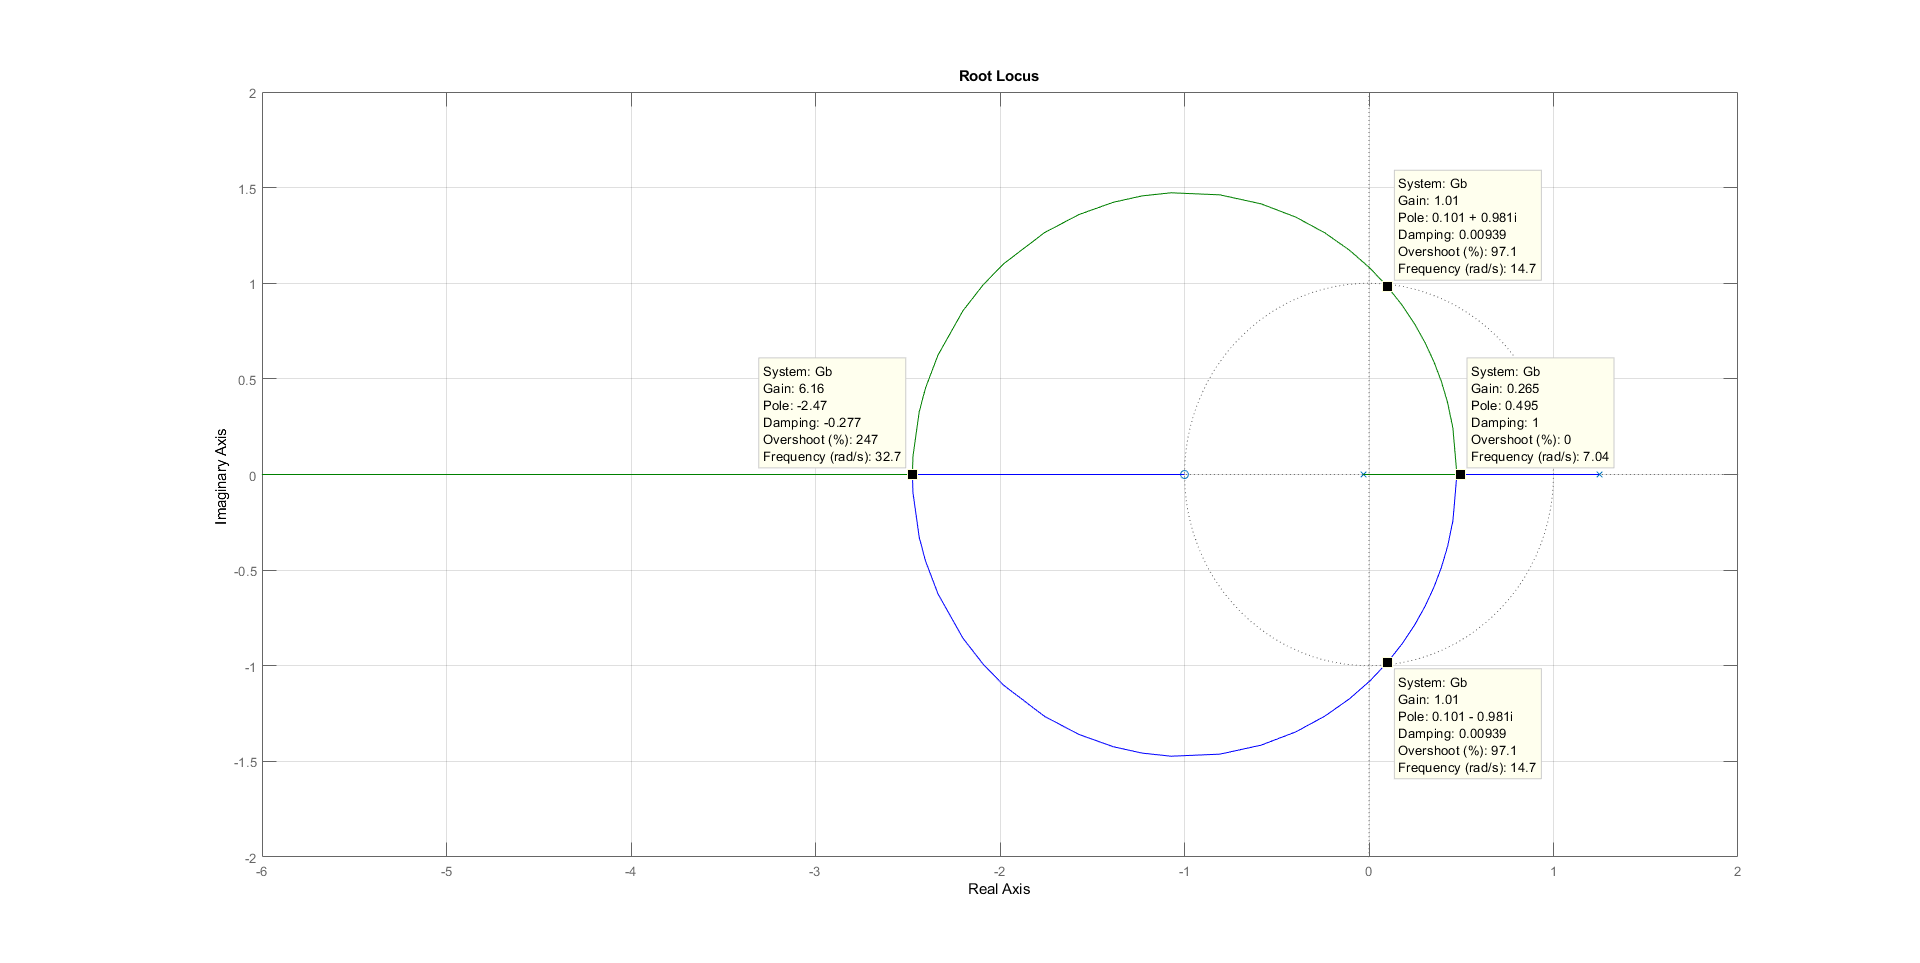
\includegraphics[width=1.0\unitlength]{images/2}
  		\caption{\label{fig:a}-}
	\end{figure}
	
	\item 
	
		$$ G_{OL}=\frac{2(0.1275)(z+1))}{(z^2+2.255z+1)+K_D(0.52)(z-1)}$$
		
		characteristic equation 
		
		$$ 1+G_{OL}=0$$
		
		or
		
		$$ (z^2+2.255z+1)+K_D(0.52)(z-1)+2(0.1275)(z+1)=0$$
		
		$$ 1 + K_d\frac{(0.52)(z-1)}{(z^2+2.255z+1)+2(0.1275)(z+1)}=0$$
		
		$$ \hat{G}_{OL}=\frac{(0.52)(z-1)}{(z^2+2.255z+1)+2(0.1275)(z+1)}$$	
		
		$$ \hat{G}_{OL}=\frac{0.52(z-1}{z^2-2z+1.255}=\frac{0.52(z-1))}{(z-1-0.5j)(z-1+0.5j)}$$
		
		Let us find break in/away points
		
		$$ 	\frac{d}{d\sigma}\frac{1}{G_{OL}(\sigma)}=z^2-z+0.745=0$$
		
		$$ \sigma_{1,2}=0,49\ \& \ 1.5$$
		
		since $\sigma=1.5$ is out of root locus, it is unnecessary
		
		\lstinputlisting[language=Matlab,firstline=17, lastline=21]{MP4_upd.m}
	
	\begin{figure}[H]
			\center
			\setlength{\unitlength}{\textwidth} 
		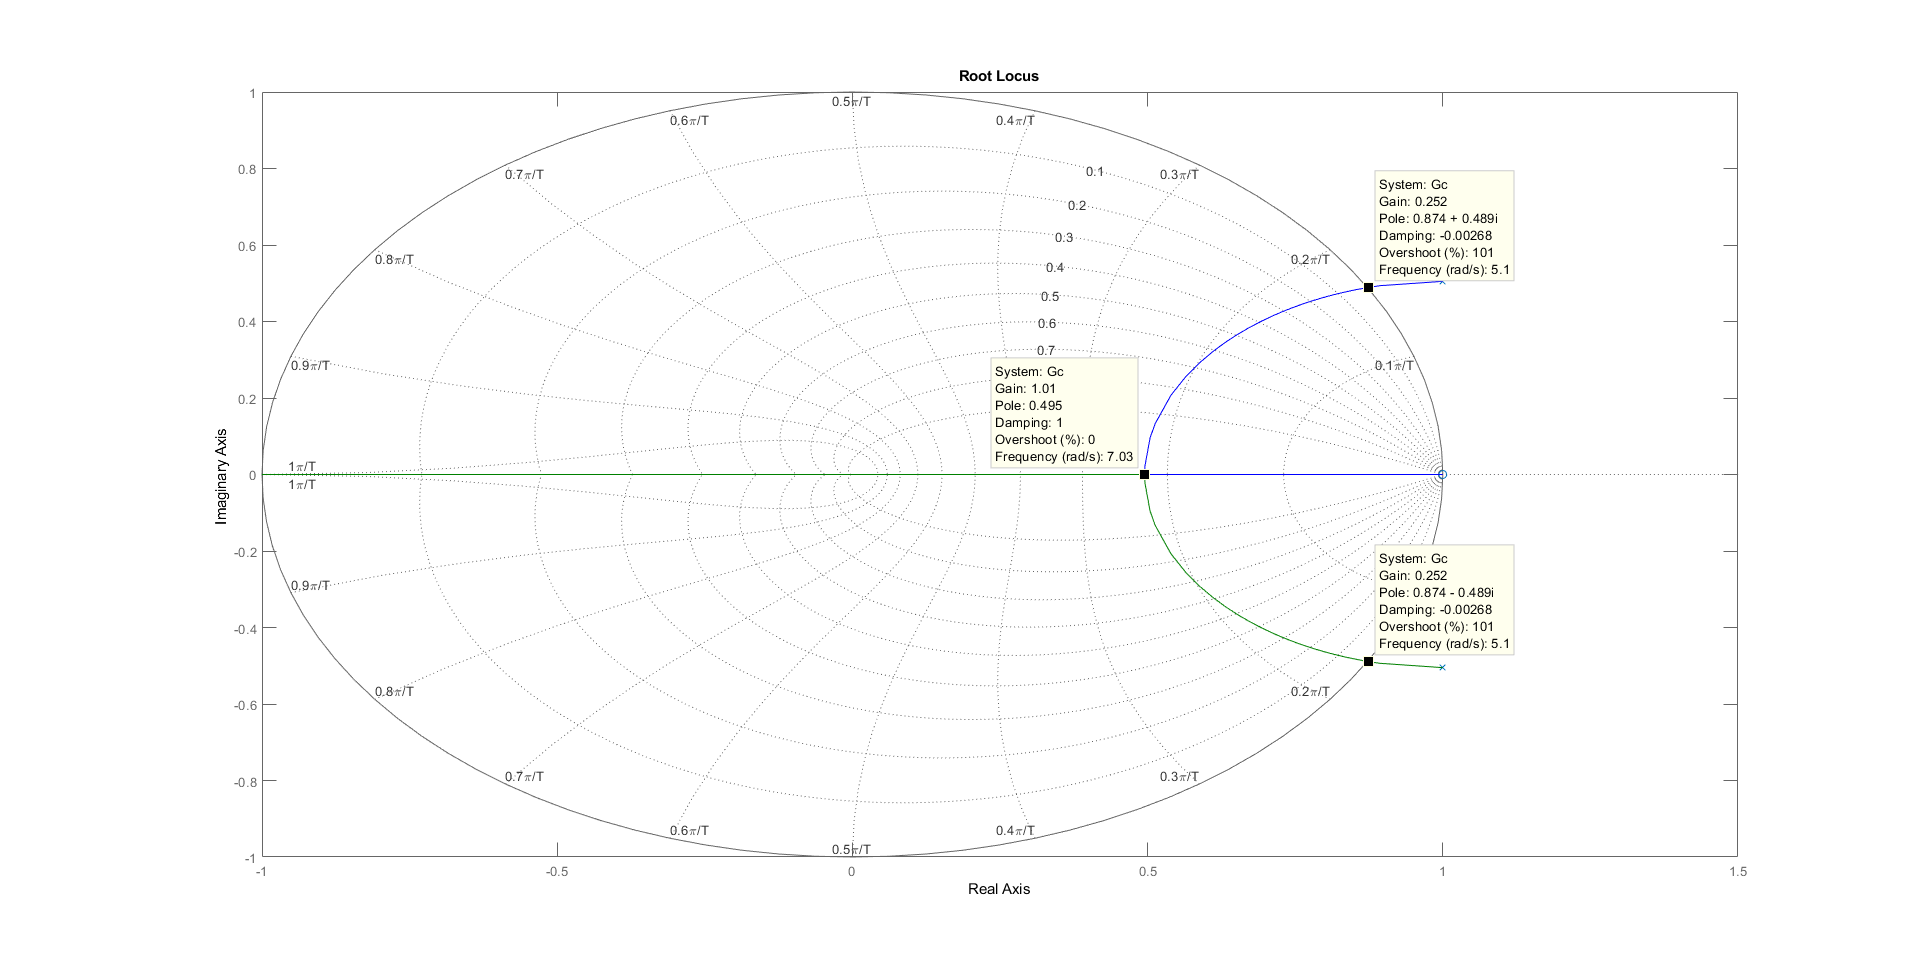
\includegraphics[width=1.0\unitlength]{images/3}
  		\caption{\label{fig:a}-}
	\end{figure}
	 

	
	
	
	\item 
	
	\begin{enumerate}
	\item -
	
		\begin{figure}[H]
			\center
			\setlength{\unitlength}{\textwidth} 
		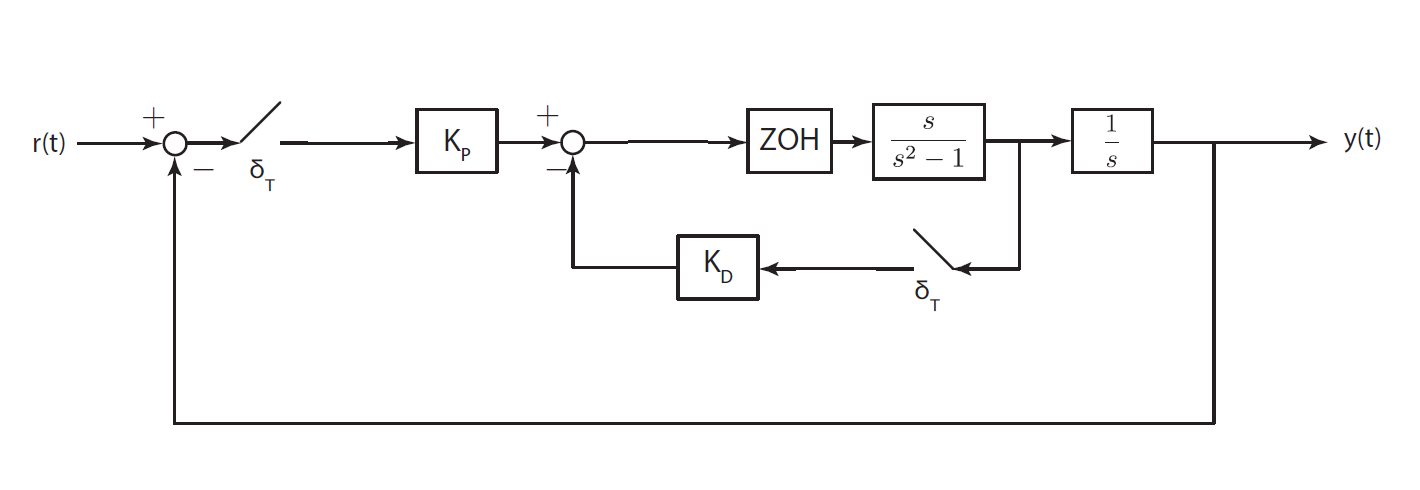
\includegraphics[width=1.0\unitlength]{images/a}
  		\caption{\label{fig:a}-}
	\end{figure}
	
		$$ e_{ss}=\lim_{ z \to 1}\frac{1+K_DG_x(z)}{1+K_DG_x(z)+K_pG_y(z)}=\frac{1}{1-K_p}$$
	
	\item -
	
		\begin{figure}[H]
			\center
			\setlength{\unitlength}{\textwidth} 
		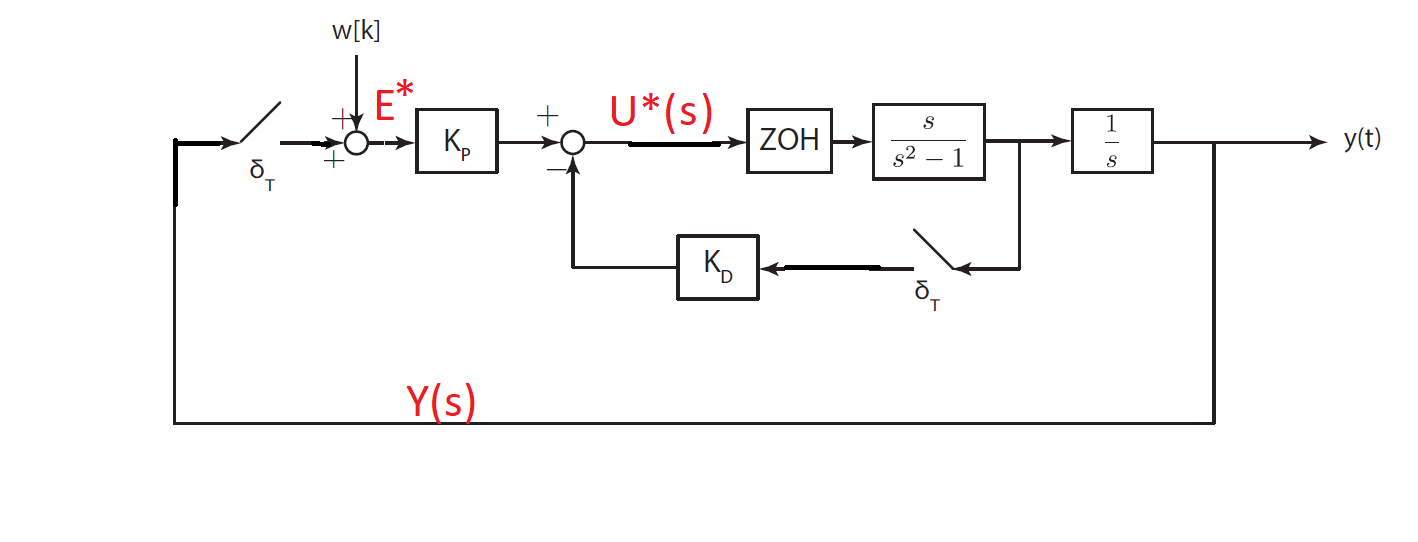
\includegraphics[width=1.0\unitlength]{images/b}
  		\caption{\label{fig:a}-}
	\end{figure}
	
		$$ U*(s)=K_pE^*(s)-U^*(s)G_x^*(s)K_d $$
		
		$$ \frac{U^*(s)}{E^*(s)}=\frac{K_p}{1+K_dG_x^*(s)}$$
		
		$$ E^*(s)=U^*(s)G_y(s)+W^*(s) $$
		
		$$ E^*(s)=\frac{K_pG_y(s)}{1+K_dG_x^*(s)}E^*(s)+W^*(s) $$
		
		$$ \frac{E^*(s)}{W^*(s)}=\cfrac{1}{1+\cfrac{K_pG_y(s)}{1+K_dG_x^*(s)}}$$
		
		$$ \frac{Y^*(s)}{U^*(s)}=G_y(s)$$
		
		$$ \frac{Y^*(s)}{E^*(s)}=\frac{K_pG_y(s)}{1+K_dG_x^*(s)} $$
		
		$$ \frac{Y^*(s)}{W^*(s)}=\cfrac{\cfrac{K_pG_y^*(s)}{1+K_dG_x^*(s)}}{1+\cfrac{K_pG_y^*(s)}{1+K_dG_x^*(s)}}=\frac{K_pG_y^*(s)}{1+K_DG_x^*(s)+K_pG_y^*(s)}$$
		
		$$ \frac{Y(z)}{W(z)}=\frac{K_pG_y(z)}{1+K_DG_x(z)+K_pG_y(z)}$$
		
		Remember that, the $G_x(z)$ and $G_Y(z)$ were found earlier (@ MP3) as
		
		$$\boxed  { G_y(z)\approx \frac{0.1275(z+1)}{z^2-2.255z+1} }$$		
	
		$$\boxed  { G_x(z)\approx \frac{0.52  \left(z-1 \right) }{z^2-2.255z+1 } }$$
		
		$$ y_ss=\lim_{z \to 1}(1-z^{-1})W(z)\frac{K_pG_y(z)}{1+K_DG_x(z)+K_pG_y(z)} $$
		
		with $ W(z)=\frac{1}{1-z^{-1}} $
		
		$$ y_{ss}=\frac{K_p\lim_{z \to 1}G_y(z)}{1+K_D\lim_{z \to 1}G_x(z)+K_p\lim_{z \to 1}G_y(z)} $$
		
		$$ \lim_{z \to 1}G_x(z)= 0$$
		
		$$ \lim_{z \to 1}G_y(z) = \frac{0.1275(2)}{1-2.255+1}=-1$$
		
		$$ y_{ss}=\frac{K_p}{K_p-1} $$
		
	
	\item -
	
		\begin{figure}[H]
			\center
			\setlength{\unitlength}{\textwidth} 
		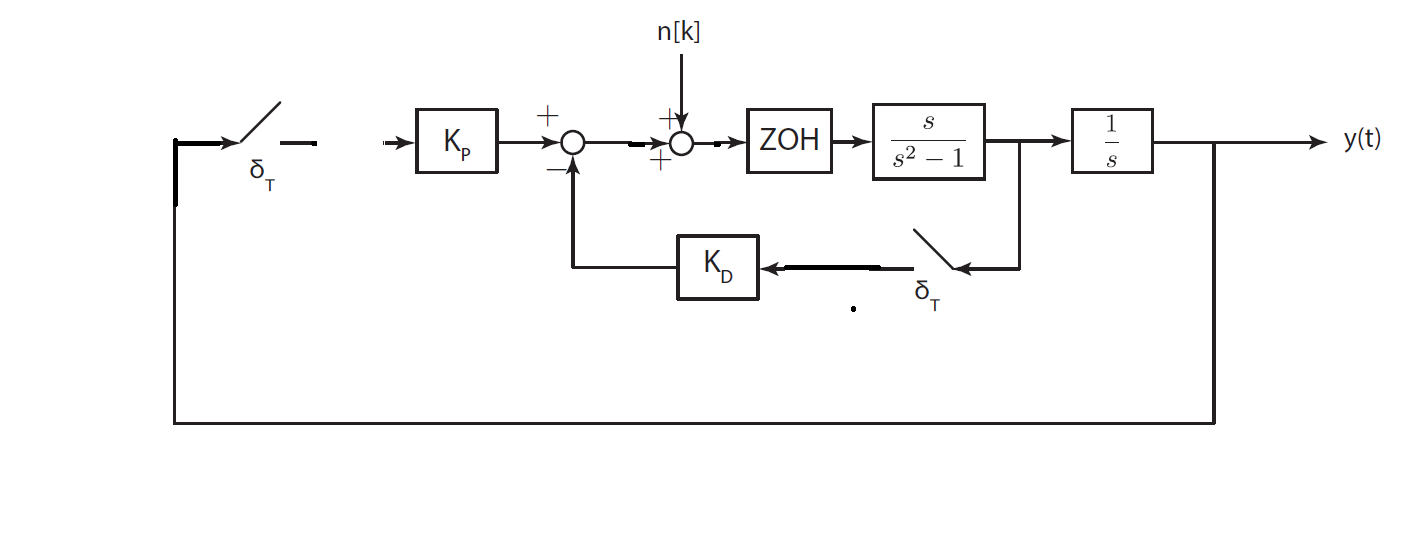
\includegraphics[width=1.0\unitlength]{images/c}
  		\caption{\label{fig:a}-}
	\end{figure}
	
	$$ e_{ss}=\lim_{ z \to 1}\frac{-K_DG_x(z)}{1+K_DG_x(z)+K_pG_y(z)}=\frac{K_D}{1-K_p}$$
	
	
	\item -

		\begin{figure}[H]
			\center
			\setlength{\unitlength}{\textwidth} 
		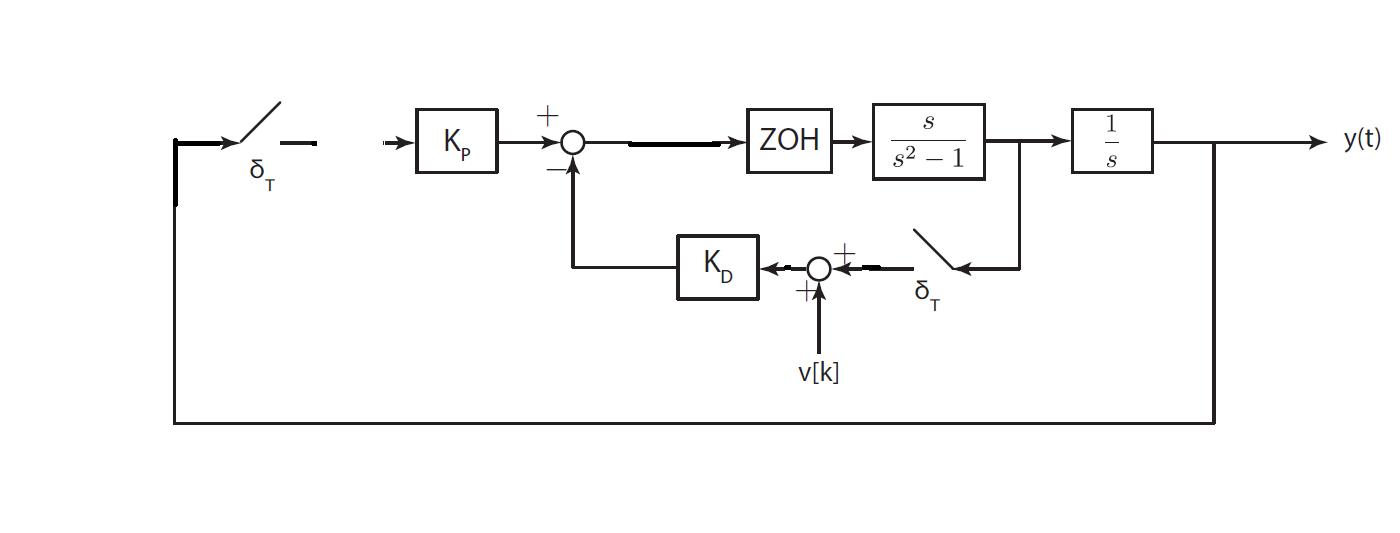
\includegraphics[width=1.0\unitlength]{images/d}
  		\caption{\label{fig:a}-}
	\end{figure}
	
	$$ e_{ss}=\lim_{ z \to 1}\frac{G_x(z)}{1+K_DG_x(z)+K_pG_y(z)}=\frac{-1}{1-K_p}$$

	\item -
	
	\begin{figure}[H]
			\center
			\setlength{\unitlength}{\textwidth} 
		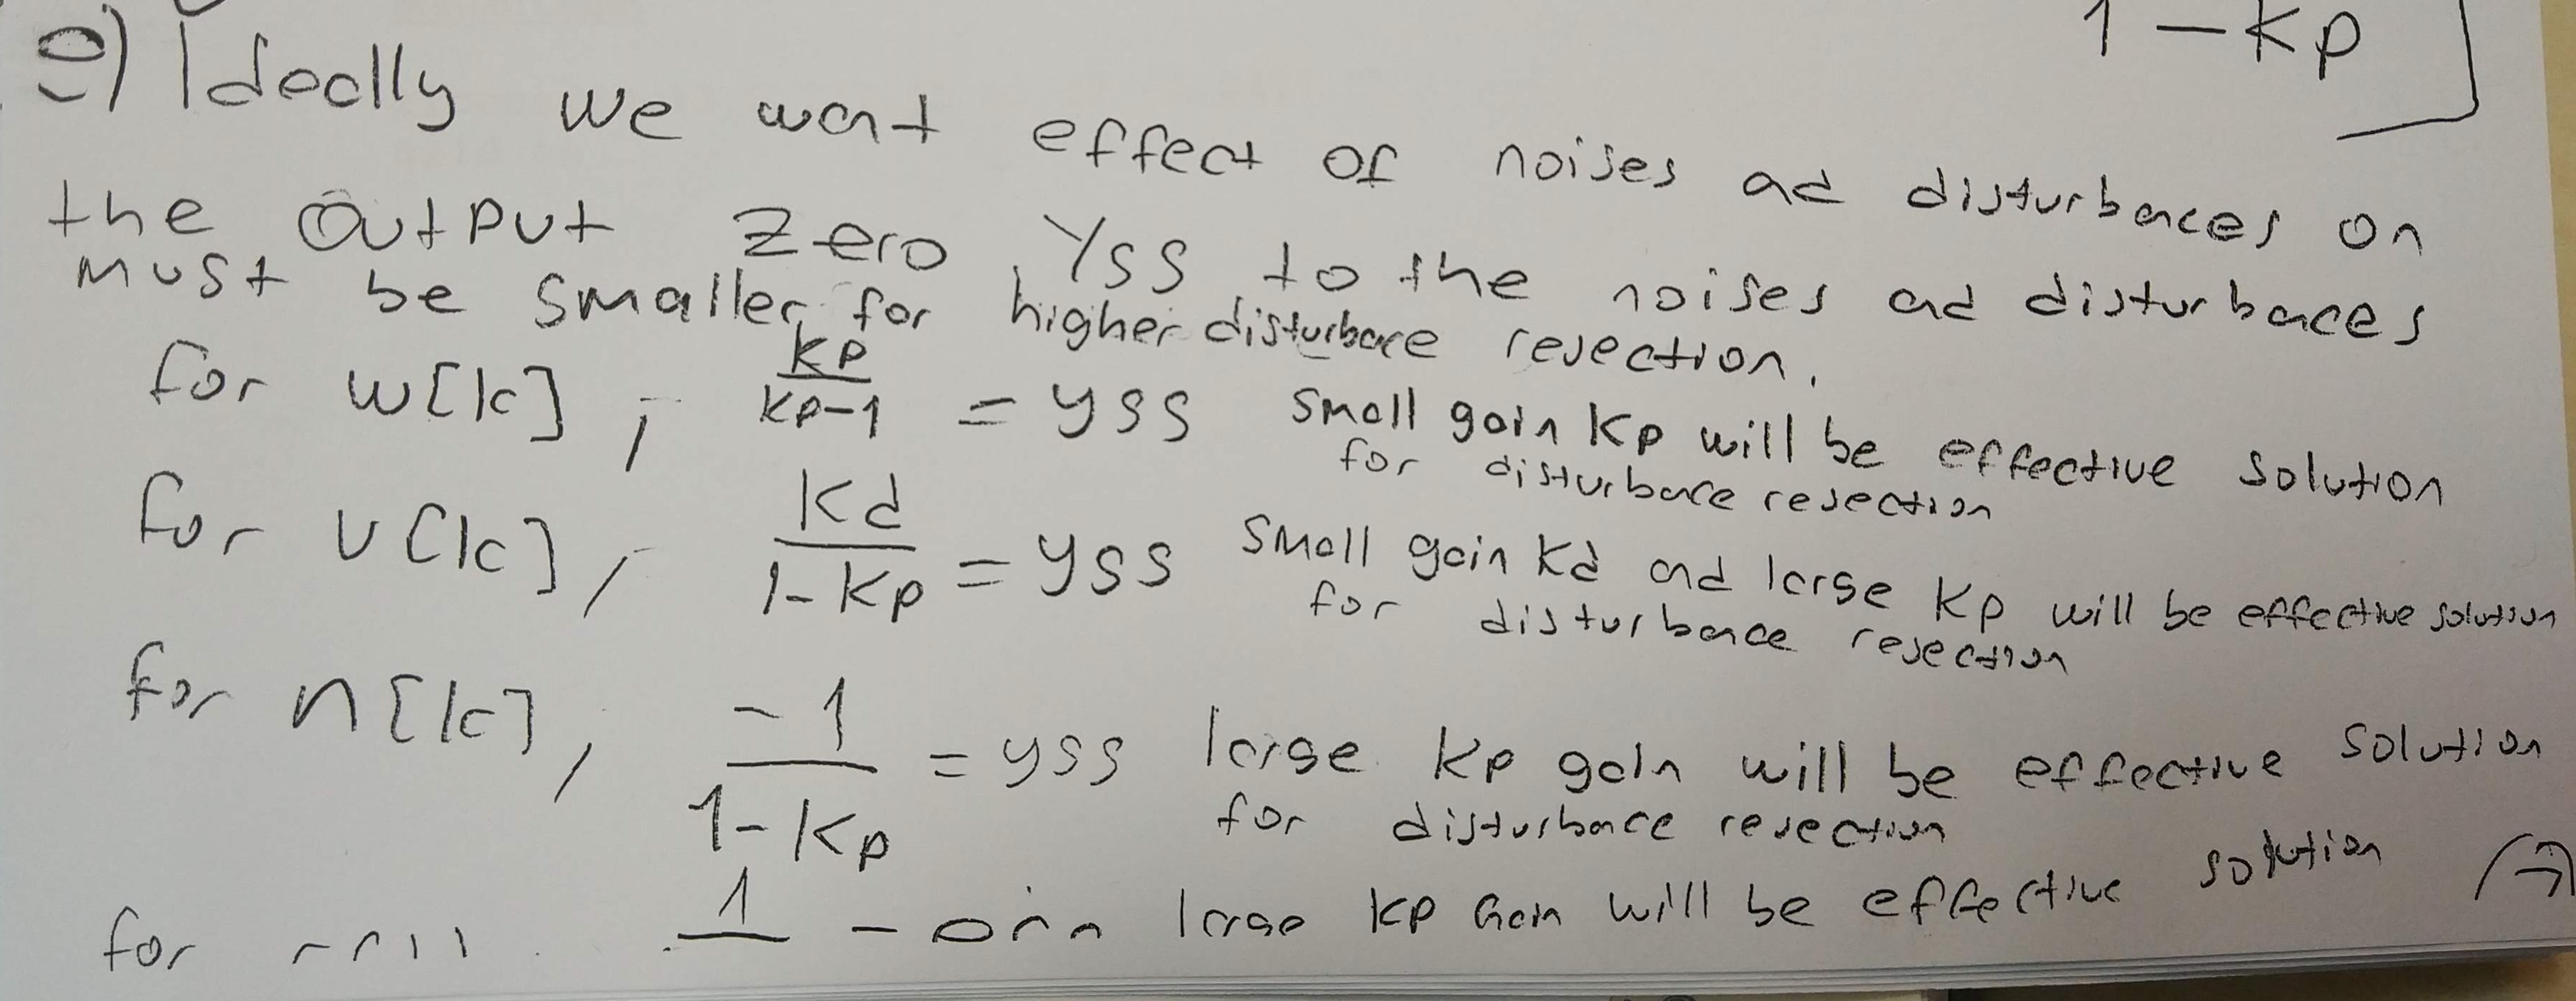
\includegraphics[width=1.0\unitlength]{images/son}
  		\caption{\label{fig:a}-}
	\end{figure}
	
	
	
	\end{enumerate}
		 	
\end{enumerate}
	
%		\newpage
%\begin{appendices}
%	\section{Source Code For Question 2}
%		\lstinputlisting[language=Matlab]{q2.m} \-\\[1cm]

%		\lstinputlisting[language=Matlab]{mydelta.m} \-\\[1cm]
%		\newpage
%	\section{Source Code For Question 3}
%		\lstinputlisting[language=Matlab]{q3.m} \-\\[1cm]
%	\section{Source Code For Question 4}
%		\lstinputlisting[language=Matlab]{q4.m} \-\\[1cm]
%				\lstinputlisting[language=Matlab,firstline=33, lastline=34]{q13.m} \-\\[1cm]
%\end{appendices}
				

%\begin{appendices}
%\section{Source Code for Matlab Part}\label{appendix}
	%%	\lstinputlisting[language=Matlab,firstline=33, lastline=34]{q13.m} \-\\[1cm]		
%\lstinputlisting[language=Matlab]{Q1.m} 


%\begin{figure}[H]
%	\setlength{\unitlength}{\textwidth} 
%	\centering
%	\begin{subfigure}{.5\textwidth}
%		\centering
		%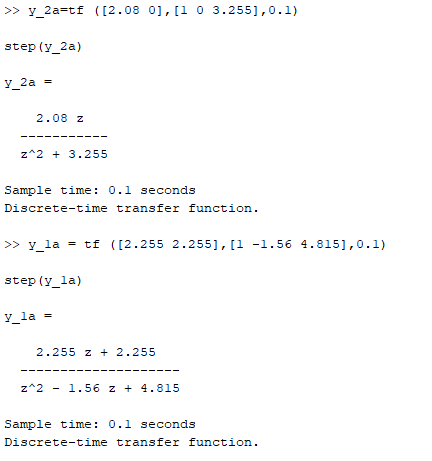
\includegraphics[width=.42\unitlength]{images/y1y2a}
%		\caption{\label{fig:y1y2a} The output for the source code for first part}
%	\end{subfigure}%
%	\begin{subfigure}{.5\textwidth}
%		\centering
%		%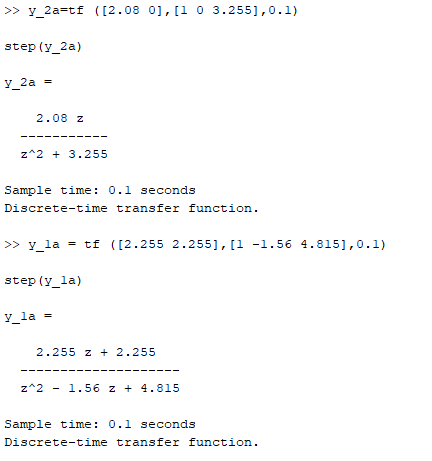
\includegraphics[width=.42\unitlength]{images/y1y2a}
%		\caption{\label{fig:y1y2a} The output for the source code for 2\nd part}
%	\end{subfigure}
%	\caption{\label{fig:y1y2ab} The output for the source code }
%\end{figure}




%\end{appendices}


\end{document}

%----samples------
%\begin{itemize}
%\item Item
%\item Item
%\end{itemize}

%\begin{figure}[H]
%\center
%\setlength{\unitlength}{\textwidth} 
%\includegraphics[width=0.7\unitlength]{images/logo1}
%\caption{\label{fig:logo}Logo }
%\end{figure}

%\begin{figure}[H]
%	\setlength{\unitlength}{\textwidth} 
%	\centering
%	\begin{subfigure}{.5\textwidth}
%  		\centering
%  		\includegraphics[width=0.48\unitlength]{images/logo1}
%  		\caption{\label{fig:logo1}Logo1 }
%	\end{subfigure}%
%	\begin{subfigure}{.5\textwidth}
%  		\centering
%		\includegraphics[width=0.48\unitlength]{images/logo2}
%  		\caption{\label{fig:logo2}Logo2}
%	\end{subfigure}
%\caption{\label{fig:calisandegree} Small Logos   }
%\end{figure}
	
%\begin{table}[H]
%  \centering
% 
%    \begin{tabular}{c|c|c}
%       $$A$$ & $$B$$ & $$C$$ \\ \hline
%       1 & 2 & 3  \\ \hline
%       2 & 3 & 4  \\ \hline
%       3 & 4 & 5  \\ \hline
%       4 & 5 & 6  
%      
%  \end{tabular}
%  \caption{table}
%  \label{tab:table}
%\end{table}
	
%\begin{table}[H]
%  \centering
% 
%    \begin{tabular}{c|c|c}
%       \backslashbox{$A$}{$a$} & $$\specialcell{ Average deviation \\ after subtracting out the  \\ frequency error }$$ & $$C$$ \\ \hline
%       \multirow{2}{*}{1} & 2 & 3  \\ \cline{2-3}
%        & 3 & 4  \\ \hline
%       3 & \multicolumn{2}{c}{4}  \\ \hline
%       4 & 5 & 6  
%      
%  \end{tabular}
%  \caption{table}
%  \label{tab:table}
%\end{table}
%-----end of samples-----